\documentclass{article}
\usepackage{amsmath,gensymb,color,graphicx,array}
\usepackage[margin=22mm]{geometry}
\newcommand{\code}[1]{\texttt{#1}}
\renewcommand{\Re}{\operatorname{Re}}
\renewcommand{\Im}{\operatorname{Im}}
\newcommand{\rtwo}{\frac{1}{\sqrt{2}}}
\newcommand{\rtd}{\frac{\delta^+}{\sqrt{2}}}
\newcommand{\rtc}{\frac{\delta^-}{\sqrt{2}}}
\newcommand{\I}{\tilde I}
\newcommand{\Q}{\tilde Q}
\newcommand{\U}{\tilde U}
\newcommand{\V}{\tilde V}
\newcommand{\J}{{\tilde E}}

\begin{document}

\section{The PIXIE fourier transform spectrometer}
PIXIE has two barrels, A and B. We can expand the electric field $\vec E^A(t)$,
$\vec E^B(t)$ that enters these barrels in terms of Jones vectors as
\begin{align}
	\vec E^A(t) &= \Re \int_0^\infty d\omega \Big(\J^A_x(\omega)\vec e_x +
		\J^A_y(\omega)\vec e_y\Big) e^{i(kz-\omega t)} \notag \\
	\vec E^B(t) &= \Re \int_0^\infty d\omega \Big(\J^B_x(\omega)\vec e_x +
		\J^B_y(\omega)\vec e_y\Big) e^{i(kz-\omega t)}
\end{align}
where $\omega$ is the angular frequency of the radiaton and $\vec \J^A(\omega)$
and $\vec \J^B(\omega)$ are (complex) Jones vectors at that
angular frequency.

After entering the barrels the light encounters polarizer A, which lets through
vertical polarization and reflects horizontal\footnote{
	Before this it encounters the primary mirror, folding flats, secondary mirror,
	and transfer mirror 1, but these lead to the same phase shifts on both
	the A and B side optical paths, so they can be neglected.}. Afer this,
the Jones vectors in left (A) and right (B) shafts are
\begin{align}
	\vec \J^{A1} &= \J^A_x \vec e_x + \J^B_y \vec e_y &
	\vec \J^{B1} &= \J^B_x \vec e_x + \J^A_y \vec e_y
\end{align}
After passing through the diagonal polarizer B, we have
\begin{align}
	\vec \J^{A2} &= \rtwo [\J^A_x+\J^B_y]\vec e_a + \rtwo[-\J^B_x+\J^A_y]\vec e_b &
	\vec \J^{B2} &= \rtwo [\J^B_x+\J^A_y]\vec e_a + \rtwo[-\J^A_x+\J^B_y]\vec e_b
\end{align}
where $\vec e_a \equiv \rtwo [\vec e_x + \vec e_y]$ and $\vec e_b
\equiv \rtwo [-\vec e_x + \vec e_y]$. The dihedral mirror then
imparts a path length difference between the two sides, advancing
A by $\frac12\Delta t$ and retarding B by $\frac12\Delta t$, which
is achieved by multiplying A by $\delta^+ = e^{-\frac12\omega\Delta t}$
and B by $\delta^- = e^{i\omega\Delta t}$:
\begin{align}
	\vec \J^{A3} &= \rtd [\J^A_x+\J^B_y]\vec e_a + \rtd[-\J^B_x+\J^A_y]\vec e_b &
	\vec \J^{B3} &= \rtc [\J^B_x+\J^A_y]\vec e_a + \rtc[-\J^A_x+\J^B_y]\vec e_b
\end{align}
Polarizer C is also diagonal.
\begin{align}
	\vec \J^{A4} &= \rtd [\J^A_x+\J^B_y]\vec e_a + \rtc [-\J^A_x+\J^B_y]\vec e_b &
	\vec \J^{B4} &= \rtc [\J^B_x+\J^A_y]\vec e_a + \rtd [-\J^B_x+\J^A_y]\vec e_b
\end{align}
And the final polarizer D is vertical. The output of this enters
the left (L) and right (R) feedhorns.
\begin{align}
	\vec \J^L = \vec \J^{A5} &= \frac12 \Big[\delta^+(\J^A_x+\J^B_y)+\delta^-(\J^A_x-\J^B_y)\Big]\vec e_x
		+ \frac12 \Big[\delta^-(\J^B_x+\J^A_y)+\delta^+(-\J^B_x+\J^A_y)\Big]\vec e_y \notag \\
		&= \big[\J^A_x\cos(\omega\Delta t/2) - i\J^B_y\sin(\omega\Delta t/2)\big]\vec e_x
		+  \big[\J^A_y\cos(\omega\Delta t/2) + i\J^B_x\sin(\omega\Delta t/2)\big]\vec e_y \\
	\vec \J^R = \vec \J^{B5} &= \frac12 \Big[\delta^-(\J^B_x+\J^A_y)+\delta^+(\J^B_x-\J^A_y)\Big]\vec e_x
		+ \frac12 \Big[\delta^+(\J^A_x+\J^B_y)+\delta^-(-\J^A_x+\J^B_y)\Big]\vec e_y \notag \\
		&= \big[\J^B_x\cos(\omega\Delta t/2) + i\J^A_y\sin(\omega\Delta t/2)\big]\vec e_x
		+  \big[\J^B_y\cos(\omega\Delta t/2) - i\J^A_x\sin(\omega\Delta t/2)\big]\vec e_y
\end{align}

\subsection{Stokes parameters}
\label{s:stokes}
After passing through all this, the light enters the feedhorns and
hits the detectors. The power deposited here can be decomposed into
Stokes parameters\footnote{The quantities with tildes are for a single plane wave.
The full Stokes parameters are obtained by integrating these. E.g. $I(\Delta t) =
	\int_0^\infty \I(\omega) d\omega$.}
\begin{align}
	\I &= \langle |\J_x|^2\rangle + \langle|\J_y|^2\rangle &
	\Q &= \langle |\J_x|^2\rangle - \langle|\J_y|^2\rangle &
	\U &= 2\Re\langle \J_x\J_y^*\rangle &
	\V &= -2\Im\langle \J_x\J_y^*\rangle
\end{align}
so we need to evaluate $P_{xx} = \langle |\J_x|^2\rangle$,
$P_{yy} = \langle |\J_y|^2\rangle$ and $P_{xy} = \langle \J_x\J_y^*\rangle$.
For the left horn\footnote{The right horn follows by symmetry: $(L,A,B)\leftrightarrow
(R,B,A)$.} we get
\begin{align}
	P^L_{xx} &= \langle \J^L_x\J^{L*}_x \rangle \notag \\
		&= \frac12\big[1+\cos(\omega\Delta t)\big]\langle\J^A_x\J^{A*}_x\rangle
		+ \frac12\big[1-\cos(\omega\Delta t)\big]\langle\J^B_y\J^{B*}_y\rangle
		- \frac{i}2\langle\J^A_x\J^{B*}_y + \J^{A*}_x\J^B_y\rangle\sin(\omega\Delta t) \notag \\
		&= \frac14\big[\I^A+\I^B+\Q^A-\Q^B + (\I^A-\I^B+\Q^A+\Q^B)\cos(\omega\Delta t) -
		4\Im(\J^A_x\J^{B*}_y)\sin(\omega\Delta t) \big] \\
	P^L_{yy} &= \frac14\big[\I^B+\I^A+\Q^B-\Q^A - (\I^B-\I^A+\Q^B+\Q^A)\cos(\omega\Delta t) -
		4\Im\langle\J^B_x\J^{A*}_y\rangle\sin(\omega\Delta t) \big ]\\
	P^L_{xy} &= \frac14\big[\U^A-\U^B - i\V^A-i\V^B + (\U^A+\U^B -i\V^A+i\V^B)\cos(\omega\Delta t)
		+2i\langle\J^A_x\J^{B*}_x+\J^B_y\J^{A*}_y\rangle\sin(\omega\Delta t)
\end{align}
Hence
\begin{align}
	\I^L &= \frac12\big[\I^A+\I^B+(\I^A-\I^B)\cos(\omega\Delta t)
		-2\Im\langle\J^A_x\J^{B*}_y+\J^B_x\J^{A*}_y\rangle\sin(\omega\Delta t) \big] \notag \\
	\Q^L &= \frac12\big[\Q^A-\Q^B+(\Q^A+\Q^B)\cos(\omega\Delta t)
		-2\Im\langle\J^A_x\J^{B*}_y-\J^B_x\J^{A*}_y\rangle\sin(\omega\Delta t) \big] \notag \\
	\U^L &= \frac12\big[\U^A-\U^B+(\U^A+\U^B)\cos(\omega\Delta t)
		-2\Im\langle\J^A_x\J^{B*}_x+\J^B_y\J^{A*}_y\rangle\sin(\omega\Delta t) \big] \notag \\
	\V^L &= \frac12\big[\V^A+\V^B+(\V^A-\V^B)\cos(\omega\Delta t)
		-2\Re\langle\J^A_x\J^{B*}_x+\J^B_y\J^{A*}_y\rangle\sin(\omega\Delta t) \big]
\end{align}
The value of the barrel cross-terms depends on whether PIXIE is in single
or double barrel mode.

\paragraph{Single barrel mode}
In single barrel mode only one barrel is exposed to the sky; the other one
observes a static calibrator object. The light entering the two barrels is
therefore uncorrelated, and all the cross-terms disappear.
\begin{align}
	\I^L &= \frac12\big[\I^A+\I^B+(\I^A-\I^B)\cos(\omega\Delta t)\big] &
	\Q^L &= \frac12\big[\Q^A-\Q^B+(\Q^A+\Q^B)\cos(\omega\Delta t)\big] \notag \\
	\V^L &= \frac12\big[\V^A+\V^B+(\V^A-\V^B)\cos(\omega\Delta t)\big] &
	\U^L &= \frac12\big[\U^A-\U^B+(\U^A+\U^B)\cos(\omega\Delta t)\big] \label{eq:single}
\end{align}

\paragraph{Double barrel mode}
In double barrel mode the two barrels are both coaligned exposed to the sky,
so they observe the same wavefront entering. As PIXIE's angular resolution is
not infinite it is sensitive to wavefronts that are off-axis by a few degrees.
Light arriving from direction $\hat n$ will hit Barrel B a time
$\tau = \hat n \cdot \vec b / c$ before barrel A, where $\vec b$ is the distance vector from
barrel A to barrel B, and $c$ is the speed of light (see~\cite{pixie_array}).
So in this case $\vec \J^B = \gamma \vec\J^A$ with $\gamma = e^{-i\omega\tau}$.
\begin{align}
	\I^L &= \I^A+\V^A\cos(\omega\tau)\sin(\omega\Delta t) &
	\Q^L &= \Q^A\cos(\omega\Delta t)-\U^A\sin(\omega\tau)\sin(\omega\Delta t) \notag \\
	\V^L &= \V^A-I^A\cos(\omega\tau)\sin(\omega\Delta t) &
	\U^L &= \U^A\cos(\omega\Delta t)-\Q^A\sin(\omega\tau)\sin(\omega\Delta t) \label{eq:double}
\end{align}
If the barrels are not perfectly collimated, or if they have asymmetric sidelobes or different beam size,
then the situation will be more complicated, as only part of the radiation that
enters the barrels will be correlated.

The leakage terms are not yet implemented in the simulator described in this
article. However, as they are all proportional to $\sin(\omega\Delta t)$ and
are therefore an antisymmetric function of the mirror stroke, they can be
easily disentangled from the main signal which is symmetric. Their absence
from the simulation should therefore impact our results meaninfully.

In the absence of the leakage terms, the signal in double barrel mode is
identical to that of single barrel mode with $(I^A,Q^A,U^A,V^A)=(I^B,Q^B,U^B,V^B)$,
so we can use the single barrel eqs~(\ref{eq:single}) in the following
without further loss of generality.

\subsection{Detector response}
PIXIE has an x and y-oriented detector in each horn. The power deposited on each
of these is
\begin{align}
	s^L_x(\Delta t)
		&= \frac14 \int_0^\infty\Big(\I^A+\I^B+\Q^A-\Q^B + (\I^A-\I^B+\Q^A+\Q^B)\cos(\omega\Delta t)\Big)d\omega \notag \\
		&= \frac14 \big[I^A+I^B+Q^A-Q^B\big]_0 + \frac14\big[I^A-I^B+Q^A+Q^B\big]_{\Delta t} \notag \\
	s^L_y(\Delta t)
		&= \frac14 \big[I^B+I^A+Q^B-Q^A\big]_0 - \frac14\big[I^B-I^A+Q^B+Q^A\big]_{\Delta t} \notag \\
	s^R_x(\Delta t)
		&= \frac14 \big[I^B+I^A+Q^B-Q^A\big]_0 + \frac14\big[I^B-I^A+Q^B+Q^A\big]_{\Delta t} \notag \\
	s^R_y(\Delta t)
		&= \frac14 \big[I^A+I^B+Q^A-Q^B\big]_0 - \frac14\big[I^A-I^B+Q^A+Q^B\big]_{\Delta t}
\end{align}
where all the quantities depend on $\Delta t$ and potentially $\tau$,
and where these are total stokes parameters, not the per-frequency ones,
e.g. $I = \int_0^\infty \I(\omega) d\omega$, and $[\ldots]_{\Delta t}$
means that the quantities within should be evaluated at the time delay in
the subscript.

Combining this with the effect of pixie's pointing on the sky,
we can express the total detector response as a function of the
sky autocorrelation functions.
\begin{align}
\vec s_\textrm{det}(t) &= \overbrace{\frac12\begin{bmatrix}
	\vec e_I+\vec e_Q & 0 \\
	\vec e_I-\vec e_Q & 0 \\
	0 & \vec e_I+\vec e_Q  \\
	0 & \vec e_I-\vec e_Q \end{bmatrix}}^\textrm{Detector response}
	\cdot
	\overbrace{\frac12\begin{bmatrix}
	1 &  M &  1 & -M \\
	M &  1 & -M &  1
	\end{bmatrix}}^\textrm{Horn response}
	\cdot
	\overbrace{\begin{bmatrix}
	R_{1t}\cdot\vec s_{\textrm{sky},A}(\hat p_{1t},0) \\
	R_{2t}\cdot\vec s_{\textrm{sky},B}(\hat p_{2t},0) \\
	R_{1t}\cdot\vec s_{\textrm{sky},A}(\hat p_{1t},\Delta t) \\
	R_{2t}\cdot\vec s_{\textrm{sky},B}(\hat p_{2t},\Delta t)
	\end{bmatrix}}^\textrm{Barrel signal}
	\label{eq:response}
\end{align}
where $\hat p_{bt}$ is the sky pointing of barrel $b$ at time $t$,
$\vec s_{\textrm{sky},b}(\hat p,\Delta t)$ is the beam-smoothed,
frequency-weighted sky autocorrelation
function Stokes vectors for the given pointing and time delay as
seen by barrel $b$
(different barrels can see different skies because one barrel may
be covered by a blackbody calibrator),
$R_{bt}$ is
a matrix that rotates the polarization basis from sky to instrument
coordinates, $M = \textrm{diag}(1,-1,-1,1)$ is a matrix that flips
the sign of linear polarization,
and $\vec e_I = (1,0,0,0)$ and $\vec e_Q = (0,1,0,0)$ are Stokes
I and Q basis vectors. PIXIE's interferometry shows up in two ways here:
The sky autocorrelation function, rather than just its intensity,
is what is measured; and the barrel signal differencing in the horn
response.

\subsection{Readout}
Of course, a real instrument does not read out data with infinite
time resolution, but as a set of discrete samples, each of which is
noisy. The PIXIE hardware will also apply a bandpass filter to avoid
aliasing and suppress low-frequency noise. Taking this into account,
we model the time-ordered data as
\begin{align}
	\vec d_i = B_{ij} \int_{t_j-\Delta t/2}^{t_j+\Delta t/2} \vec s_\textrm{det}(t) \textrm{d}t + \vec n_i
\end{align}
where $i$ is the sample index, $B$ is the bandpass filter, $\Delta t$ is the sample
interval and $\vec n_i$ is the noise in sample $i$. We implement this
sample integral by using Gaussian quadrature with $N_\textrm{sub}$ sub-samples,
with a typical value of $N_\textrm{sub}$ being 9. See section~\ref{s:accuracy}
for a discussion of the effect of the number of sub-samples.

For the bandpass filter we used a Butterworth bandpass filter.
\begin{align}
	B(f) &= \Big(1+\Big[\frac{f}{0.01\textrm{Hz}}\Big]^{-5}\Big)^{-1}
		\Big(1+\Big[\frac{f}{100\textrm{Hz}}\Big]^{5}\Big)^{-1}
\end{align}

\section{Pointing}
PIXIE will orbit at the Sun-Earth L2 point, placing it in the ecliptic, with
a heliocentric ecliptic latitude $b=0$ and longitude $l=l_0 +
360\degree\frac{t-t_0}{T_\textrm{orbit}}$ with $T_\textrm{orbit} = 1\textrm{year}$.
As it orbits it scans great circles
perpendicular to the direction towards the sun, with a linearly increasing scan angle
$\alpha_\textrm{scan} = \alpha_{\textrm{scan},0} + 360\degree \frac{t-t_0}{T_\textrm{scan}}$.
To form an actual great circle the scan axis does not
move continuously with $b$, but updates in steps after each circle has been completed:
$\alpha_\textrm{orbit} = l_0 + 360\degree\left\lfloor\frac{t-t_0}{T_\textrm{scan}}\right\rfloor\frac{T_\textrm{scan}}{T_\textrm{orbit}}$.
During each scan the the telescope spins around around its boresight to modulate
the observed polarization and reject systematics: $\alpha_\textrm{spin} =
\alpha_{\textrm{spin},0} + 360\degree\frac{t-t_0}{T_\textrm{spin}}$. And finally,
while it is spinning the dihedral mirror sweeps backwards and forwards at constant
speed, varying the path length time difference in the fourier transform spectrometer
by $\Delta t = A_\textrm{delay}\textrm{triangle}\Big(\frac{t-t_0}{T_\textrm{stroke}}\Big)$,
with $A_\textrm{delay} = 10.40303 \textrm{mm}/c$ for the purposes of this paper, but
varying somewhat by observing mode in the real experiment, and with
$\textrm{triangle}(x)$ being the triangle wave with period 1, mean 0 and a zero
crossing at $x=0$.

To allow PIXIE mapmaking to use fast fourier transform methods, the stroke, spin
and scan periods will be synchronized such that there is an integer number of
strokes in a spin, and an integer number of spins in a scan. We will use the
values $T_\textrm{spin} = 60 \textrm{s}$, $T_\textrm{stroke} = T_\textrm{spin}/8 =
7.5 \textrm{s}$, $T_\textrm{scan} = 384 T_\textrm{spin} = 384 \textrm{min}$ here.
The TOD simulator purposefully does not depend on integer ratios to be able
to investigate the consequences of small deviations from integer ratios.

In order to speed up our simulations we will modify the scanning pattern we
simulate in one important respect. The actual L2 obital
period given above results in about 1370 scans per orbit, which results in
7.6 scans per PIXIE beam FWHM on the equator after half an orbit. We avoid
this oversampling by simulating a faster $T_\textrm{orbit} = 384 T_\textrm{scan}$.

A barrel-to-sky rotation matrix that implements this pointing model is
\begin{align}
	R_\textrm{tot}(b,t)  &= R_\textrm{orient}(t)R_\textrm{barrel}(b) \\
	R_\textrm{orient}(t) &= R_z\big(\alpha_\textrm{orbit}(t)\big)
		R_y\Big(\frac\pi2-\alpha_\textrm{eclip}\Big)
		R_z\big(\alpha_\textrm{scan}(t)\big)R_y\Big(\frac\pi2-\alpha_\textrm{open}\Big)
		R_z\big(\alpha_\textrm{spin}(t)\big) \\
	R_\textrm{barrel}(b) &= R_z\big(\Delta\phi(b)\big)R_y\big(\Delta\theta(b)\big)R_z\big(\Delta\psi(b)\big) \label{eq:barrel}
\end{align}

Here $R_\textrm{barrel}(b)$ represents the orientation of barrel $b$ relative
to the spacecraft. Fiducially $R_\textrm{barrel} = 1$ for both barrels, but
we include this rotation to be able to support misaligned barrels or more
complicated beams. $R_\textrm{orient}(t)$ represents PIXIE's orientation
in space at time $t$, and in addition to the angles described above includes
$\alpha_\textrm{eclip}$ and $\alpha_\textrm{open}$, which represent the
offset of PIXIE's orbital plane from the ecliptic and the opening angle
offset (to support non-great-circle scans), both of which are fiducially 0.
$R_y(\theta)$ and $R_z(\theta)$ are rotations around the $y$ and $z$ axes
by an angle $\theta$.

$R_\textrm{tot}$ encodes both the sky coordinates and polarization rotation.
\begin{align}
	x_i &= R_\textrm{tot,xi} & y_i &= R_\textrm{tot,yi} & p_i &\equiv z_i = R_\textrm{tot,zi} \\
	l        &= \tan^{-1}(p_y/p_x)  &
	b        &= \tan^{-1}\Big(\frac{p_z}{\sqrt{p_x^2+p_y^2}}\Big) &
	\gamma   &= \tan^{-1}\Big(\frac{x_z}{p_y x_x - p_x x_y}\Big)
\end{align}
with all the above being a function of the barrel index and time.
$\hat p = (p_x,p_y,p_z)$ is the pointing vector and $\gamma$ is the
polarization basis rotation, and corresponds to a Stokes rotation
matrix
\begin{align}
	R &= \begin{bmatrix}
		1 & 0 & 0 & 0\\
		0 & \cos(2\gamma) & -\sin(2\gamma) & 0\\
		0 & \sin(2\gamma) & \cos(2\gamma) & 0 \\
		0 & 0 & 0 & 1
	\end{bmatrix}
\end{align}

%	p_{bt,i} &= R_{\textrm{tot,3i}}(b,t) \\

\section{Evaluating the sky autocorrelation function at the observed location}
As PIXIE observes the sky it mesures the autocorrelation function of the
radiation coming from the points it scans past. To simulate the PIXIE signal
we therefore need to be able to evaluate the I, Q and U autocorrelation
functions
\footnote{We're ignoring V polarization here. See section~\ref{s:stokes}.}
at an arbitrary point $\hat p$ on the sky for an arbitrary phase
delay $\Delta t$ for each component that makes up the sky (CMB, dust, etc.).

\subsection{Approaches that don't work}
\label{s:autocorr-problems}
A straightforward and general way of doing this would be to precompute the
full-sky autocorrelation function: Evaluate the full-sky spectrum at equi-spaced
frequencies; apply the beam to each frequency map and scale each frequency by
the instrument's frequency response; and Fourier transform the result
to get a (pixelized version of) the full-sky autocorrelation function. To read off
the value at a general $(\hat p, \Delta t)$ one would then do an interpolated lookup
in this $N_\textrm{pix}$ by $N_\textrm{delay}$ data cube. This approach has the
advantage of being able to handle frequency-dependent beams, which are otherwise
very hard to implement. However, in order to be able to investigate the effect
of sub-resolution features (both spectrally and spatially) this data cube would
need to be pixelized at many times higher resolution than the PIXIE output map.
This made the memory requirements of this approach prohibitively high. For example,
for $0.1\degree$ spatial resolution and 5000 frequency bins, storing the full-sky
autocorrelation function would need about 700 GB of RAM.

If one assumes a frequency-independent beam, which should be a good approximation
for PIXIE, and if the spectrum can be written as a linear sum of a a smaller
number of spatial templates, then it's sufficient to apply the beam to those
templates rather than the spectrum itself. This
decouples the spatial and spectral dimensions, making it possible to evaluate the
spectrum in one pixel independently of the rest of the sky.

With this, we could
imagine the following approach: For each sample, interpolate the spectrum parameters
at $\hat p$, then evaluate the whole spectrum, apply the frequency response,
fourier transform it,
and interpolate the value for $\Delta t$. In our example above, this would reduce
the RAM requirements by a factor of 5000. But it would introduce another prohibitive
cost: The need to evaluate the spectrum at thousands of frequencies and fourier transform
these for every sample in the TOD.\footnote{
A hybrid approach between these two would be to precompute the autocorrelation function
for a chunk of the sky around the current sample, and reuse that for subsequent samples
until a sample falls outside the chunk, and then precompute a new chunk. We investigated
this in the hopes of being able to support frequency-dependent beams, but found that
edge effects and the flat-sky-approximation needed to perform beam-smoothing on a small
patch did not result in the required accuracy. This may still be a good approach for
frequency-independent beam simulations, though.}

\subsection{Autocorrelation by Taylor expansion}
In the end, we went for a Taylor expansion approach: The autocorrelation function
is evaluated as a perturbation around a different but similar
precomputed autocorrelation function. This is done differently for each sky component.

\subsubsection{CMB}
Taking into account the instrument's frequency response $\rho(\nu)$, PIXIE
observes the CMB with the spectrum
\begin{align}
I^\textrm{CMB}_{\nu,I}(\hat p, \nu) &= \rho(\nu)B_\nu(\nu, T(\hat p)) = \frac{2h\nu^3\rho(\nu)}{c^2}\frac{1}{e^{\frac{h\nu}{kT(\hat p)}} - 1}
\end{align}
Here the $I$ subscript indicates the Stokes parameter, and $T(\hat p)$ is the
CMB temperature at pointing $\hat p$.
Including the doppler dipole, T only has a contrast of order $10^{-3}$, so a Taylor
expansion in T will converge rapidly. Our goal is $<10^{-9}$ relative error, so an
expansion to 3rd order, which should give order $10^{-12}$ error, should be sufficient.
The expansion is
\begin{align}
	I^\textrm{CMB}_{\nu,I}(\hat p, \nu) &= f_0(\nu) + f_1(\nu) \Delta T + \frac12 f_2(\nu) \Delta T^2 + \frac16 f_3(\nu) \Delta T^3
\end{align}
where
\begin{align*}
	f_0 &= p(g_0-1)^{-1}    & g_0 &= e^{a/T_0} \\
	f_1 &= pf_0^2 g_1       & g_1 &= -g_0 a/T_0^2 \\
	f_2 &= p(-2 f_0 f_1 g_1 - f_0^2 g_2) &
	g_2 &= a(2 g_0-T_0 g_1)/T_0^3 \\
	f_3 &= p(-2 f_1^2 g_1 - 2f_0 f_2 g_1 - 4 f_0 f_1 g_2 - f_0^2 g_3) &
	g_3 &= -(3/T_0 + a/T_0^2)g_2 + a g_1/T_0^3
\end{align*}
and where $p = \frac{2h\nu^3\rho(\nu)}{c^2}$, $a = h\nu/k$ and $\Delta T(\hat p) = T(\hat p)-T_0$ with $T_0 = 2.725$K. 

The autocorrelation function is simply the cosine transform\footnote{
We implemented the cosine transform using a discrete cosine transform with a
sample interval of 0.5 GHz and a max frequency of 6.8 THz.} of the spectral power
density,
\begin{align}
	I_{\Delta t}(\Delta t) &= \int_{0}^\infty I_\nu(\nu) \cos(2\pi\nu\Delta t) d\nu
	\equiv \bar I_\nu(\Delta t)
\end{align}
where $\bar{x}$ indicates the cosine transform of $x$.
{\color{red}This is confusing. Tilde quantities are consistently
in frequency space in the interferometry section, but here the visually
similar bars indiate the cosine transform of a frequency space quantity
into a real space quantity.}
Applying this to the Taylor expansion, we get
\begin{align}
I^\textrm{CMB}_{\Delta t,I}(\hat p,\Delta t) &= \bar f_0(\Delta t) + \bar f_1(\Delta t) \Delta T + \frac12 \bar f_2(\Delta t) \Delta T^2 + \frac16 \bar f_3(\Delta t) \Delta T^3
\end{align}
Hence, we can compute the autocorrelation for any $\hat p,\Delta t$ if we simply precompute
the four position-independent functions $\{f_i\}$.\footnote{
If we had not needed to support the frequency response of the instrument,
we could have avoided the Taylor expansion by absorbing variation in $T$
into rescaling of $v$. Sadly, PIXIE has significant damping at high frequency,
so this approach does not work.} Evaluating the CMB autocorrelation at ($\hat p,\Delta t$)
is hence reduced to being able to evaluate a sampled version of $\{f_i\}$
at (non-sample) position $\Delta t$ and
the full-sky pixelized map $\Delta T$ at (non-pixel) position $\hat p$.
We perform both of these using (bi-)cubic spline interpolation
from \code{numpy.ndimage.map\_coordinates}.

The CMB has frequency-independent polarization,
so the $Q,U$ autocorrelation functions can be derived from $I$ by scaling them by
the local $Q,U$ polarization fractions. I.e. $I^\textrm{CMB}_{\Delta t,Q|U}(\hat p,\Delta t) = I^\textrm{CMB}_{\Delta t,I}(\hat p,\Delta t) \frac{I^\textrm{CMB}_{\textrm{ref},Q|U}(\hat p)}{I^\textrm{CMB}_{\textrm{ref},I}(\hat p)}$.

The input CMB map $\Delta T,Q,U$ was simulated by drawing random, Gaussian
T,E,B and $\phi$ spherical harmonics coefficients from a typical CMB power spectrum
as output by CAMB\footnote{The spectrum used is provided in the file \code{
	inputs/cl\_lensinput.dat}.} and projecting them on a sky with $0.1\degree$
pixels in equirectangular (CAR) projection using the \code{libsharp} Spherical
Harmonics Transform library \cite{libsharp}. The lensing potential $\phi$ was then used to
lens the T, Q and U maps. We then added the 2.725 K CMB monopole to the T
component before doppler boosting the sky\footnote{$\beta=0.0012301$ towards
ecliptic coordinates $l=171.646$, $b=-11.141$.}
to account for our motion relative to the CMB, resulting in the CMB dipole.

\subsubsection{Dust}
We model the dust as a modified blackbody with constant
$T=19.6$K and $\beta=1.59$, but varying opacity. The observed spectrum is thus
\begin{align}
I^\textrm{dust}_{\nu,i}(\hat p,\nu) &= A_i(\hat p) \frac{h\nu^{3+\beta}\rho(\nu)}{c^2}\frac{1}{e^{\frac{h\nu}{kT}}-1} \equiv A_i(\hat p) f_{0\beta}(\nu)
\end{align}
for $i \in \{I,Q,U\}$. Here the prefactor $A_i(\hat p)$ encodes the position-dependent
dust opacity and polarization.
Since $T$ and $\beta$ are constant, the frequency-dependent part of this spectrum is
already position-independent, so we don't actually need to Taylor-expand in this case.
We just need to precompute a single autocorrelation shape which is rescaled for each
pointing.
\begin{align}
I^\textrm{dust}_{\Delta t,i}(\hat p,\Delta t) &= A_i(\hat p) \bar f_{0\beta}(\Delta t)
\end{align}
This will need to be modified for more complicated dust models. If $T$ or $\beta$
only change slightly, then the Taylor expansion approach can be used. For more
substantial variation, a better approach may be to model it as several dust components,
each with fixed parameters.

The input dust map was simulted using the Planck Sky Model \cite{psm} code \code{PySM}
of a thermal dust-only sky evaluated at 600 GHz (with no bandpass).
This was computed at HEALPix $N_\textrm{side} = 512$, but the polarization
map \code{PySM} produces is limited to $2\degree$ resolution due to the limited
resolution of the Planck polarized dust maps it uses as input. This HEALPix map
was then repixelized to $0.1\degree$ equirectangular (CAR) pixelization in
ecliptic coordinates by computing its spherical harmonics coefficients,
projecting these onto CAR, and then rotating from galactic to ecliptic coordinates
using bicubic spline interpolation and rotating the polarization vectors to compensate.

\subsubsection{Other components}
The results reported here are based on simulations that only include CMB and dust,
but other components such as synchrotron, free-free, CO, AME, etc. can be implemented
in a similar vein as above, as long as they can be approximated as a sum of
constant-spectral-shape components or can be Taylor-expanded to sufficient accuracy.

\subsubsection{The PIXIE frequency response}
PIXIE's frequency response is limited above 1-2 THz by the roughness of the mirrors.
We model this as $\rho(\nu) = e^{-\left[\frac{\nu}{1.5\textrm{THz}}\right]^2}$.

\section{Beams and sidelobes}
PIXIE's beam will be approximately frequency-independent and approximately
top-hat shaped, but we will here approximate it with a Gaussian
with a FWHM of $1.9\degree$. As discussed in section~\ref{s:autocorr-problems},
a frequency-independent beam is much cheaper to implement than a frequency-dependent
one as long as the spectrum maps are linear functions of a small number of input
maps. For our dust model this is simple - the spectrum is proportional
to a single spatially varying dust opacity map, so it is sufficient to apply the
beam to that map.

\subsection{A small error in the CMB beam treatment}
The CMB, on the other hand, is modeled as a 4th order Taylor
expansion in $\Delta T$, so in this case we should smooth each power of $\Delta T$
individually. We currently \emph{do not do this}. Instead, we simply smooth
the input $\Delta T$, as one usually does when simulating CMB maps. This reduces
the accuracy of our Taylor expansion, and should be fixed in a future release.
However, this is not as serious as one might fear.
\begin{enumerate}
	\item The main reason why we go to 4th order is the $O(10^{-3})$ CMB dipole,
		but the dipole is practically unaffected by the beam. The beam-relevant
		scales are much lower, at $O(10^{-5})$. The first incorrect correction
		term is the second order, which is down by another such factor, giving
		a relative accuracy of $10^{-5}$ for T, E and B perturbations. This is
		dwarfed by cosmic variance and noise for all PIXIE scales.
	\item The same beam incorrect smoothing is used when evaluating the accuracy of the
		recovered maps. These errors therefore cancel, and the difference maps and
		error plots in the results section are identical to those we would have gotten
		if this error had not been made.
\end{enumerate}

\subsection{Sidelobes and asymmetric beams}
So far we've assumed that the beam is isotropic and position-independent,
so it can be implemented by a one-time smoothing of the maps. A full
implementation of general beam shapes would be very expensive, as it
requires an integral over (part of) the sky for every sample generated.
However, we can capture all the interesting effects of complicated beams
by expanding them as a series of symmetric beams with different pointing
offsets. For example, a slightly elliptical beam can be approximated as
the sum of two slightly offset symmetric beams.
We implement this by replacing every evaluation of the sky autocorrelation
function with a sum over such evaluations for each beam component.
Each such beam component is defined by specifying
$\Delta\phi$ and $\Delta\theta$ (see eq.~(\ref{eq:barrel})),
a beam profile, and a Muller matrix which encodes its
intensity and leakage properties.

\section{Results}

\begin{figure}
	\centering
	\hspace*{-15mm}\begin{tabular}{rm{56mm}m{54.4mm}m{56mm}}
		& \hspace{32mm}T & \hspace{32mm}Q & \hspace{32mm}U \\
		CMB &
		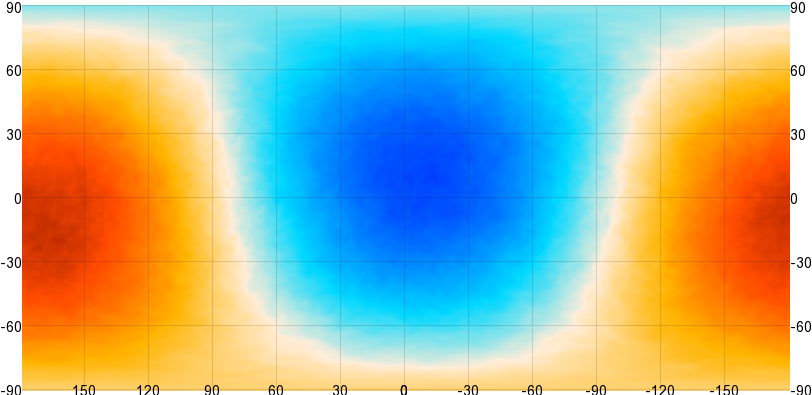
\includegraphics[height=28mm,clip,trim=0 8mm 7.5mm 0]{plots/sim_freqmap_58GHz_1_0.png} &
		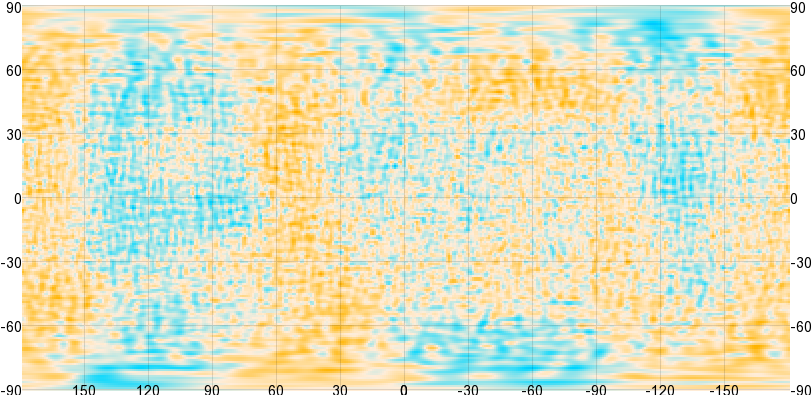
\includegraphics[height=28mm,clip,trim=7.5mm 8mm 7.5mm 0]{plots/sim_freqmap_58GHz_1_1.png} &
		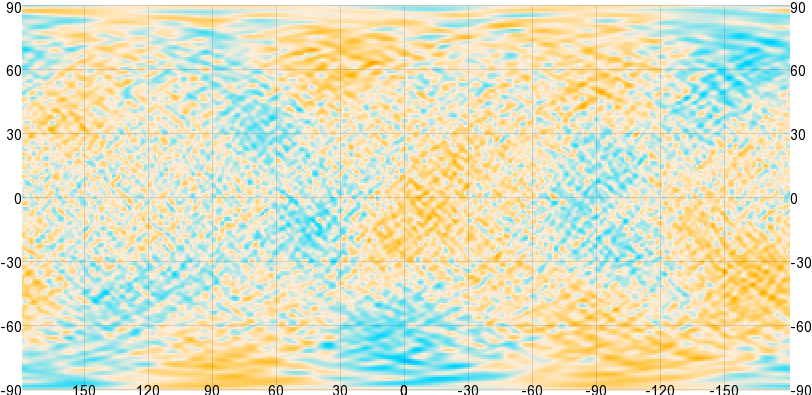
\includegraphics[height=28mm,clip,trim=7.5mm 8mm 0 0]{plots/sim_freqmap_58GHz_1_2.png} \\
		Dust &
		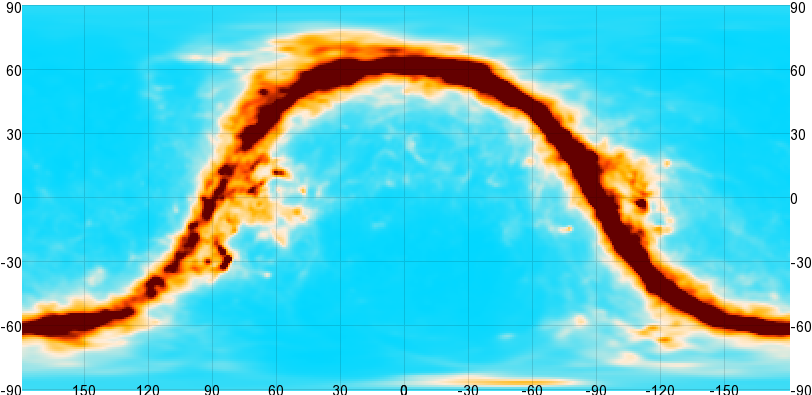
\includegraphics[height=28mm,clip,trim=0 8mm 7.5mm 0]{plots/sim_freqmap_58GHz_2_0.png} &
		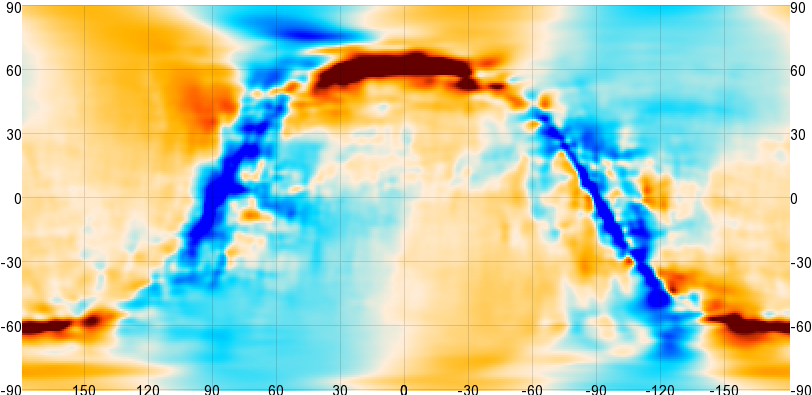
\includegraphics[height=28mm,clip,trim=7.5mm 8mm 7.5mm 0]{plots/sim_freqmap_58GHz_2_1.png} &
		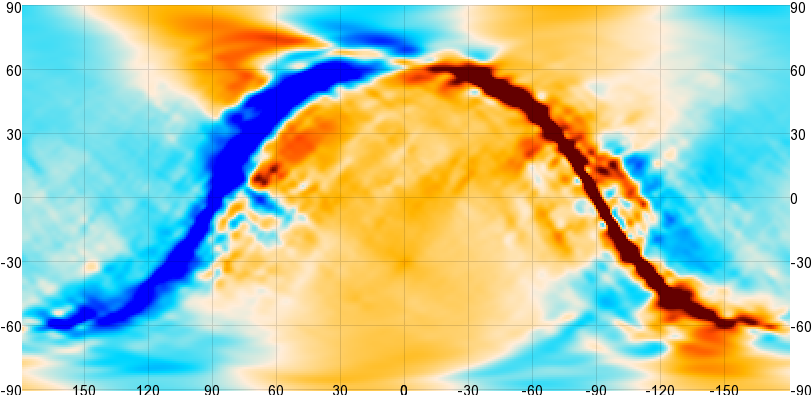
\includegraphics[height=28mm,clip,trim=7.5mm 8mm 0 0]{plots/sim_freqmap_58GHz_2_2.png} \\
		Total &
		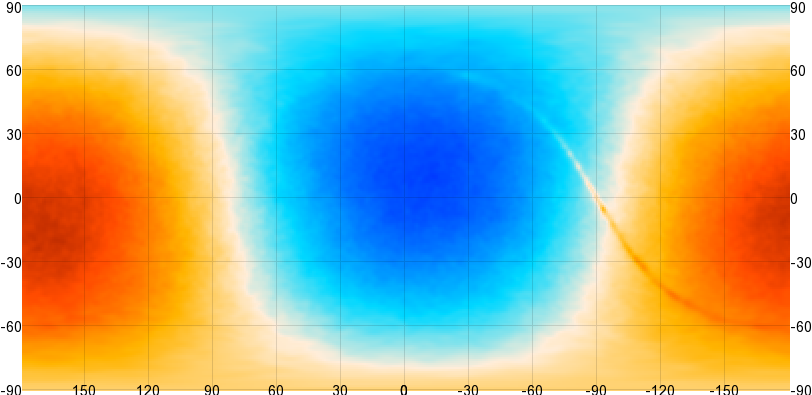
\includegraphics[height=29.7mm,clip,trim=0 0mm 7.5mm 0]{plots/sim_freqmap_58GHz_0_0.png} &
		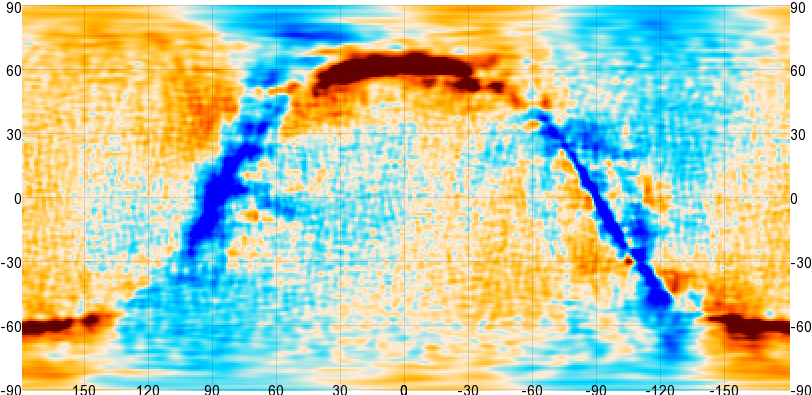
\includegraphics[height=29.7mm,clip,trim=7.5mm 0mm 7.5mm 0]{plots/sim_freqmap_58GHz_0_1.png} &
		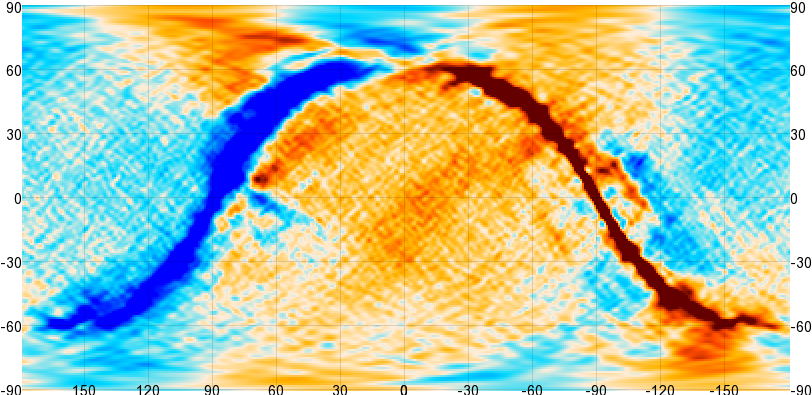
\includegraphics[height=29.7mm,clip,trim=7.5mm 0mm 0 0]{plots/sim_freqmap_58GHz_0_2.png}
	\end{tabular}
	\caption{The input beam-smoothed sky model evaluated at 58 GHz in the CAR
	projection in ecliptic coordinates. The color range is
	$\pm 400$ kJy/sr in T and $\pm 200$ Jy/sr in P, except for dust T where it is
	$\pm 5$ kJy/sr. The mean has been subtracted in each map for plotting purposes.}
\end{figure}

\begin{figure}
	\centering
	\begin{tabular}{cc}
		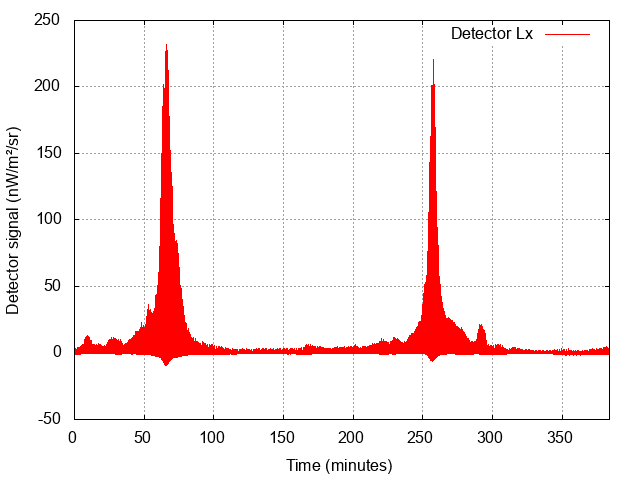
\includegraphics[width=0.48\textwidth,trim=8mm 0 0mm 0mm]{plots/tod000_full.png} &
		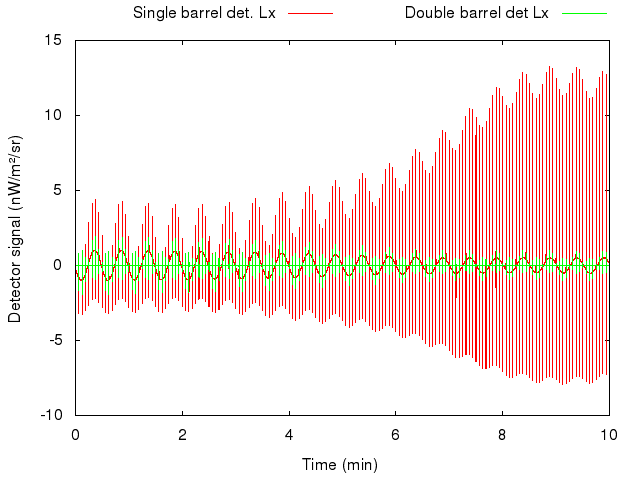
\includegraphics[width=0.48\textwidth,trim=8mm 0 0mm 0mm]{plots/tod000_10min.png} \\
		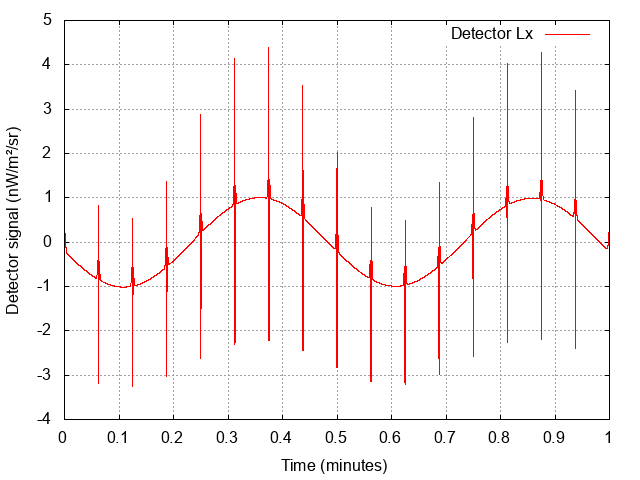
\includegraphics[width=0.48\textwidth,trim=8mm 0 0mm 0mm]{plots/tod000_1min.png} &
		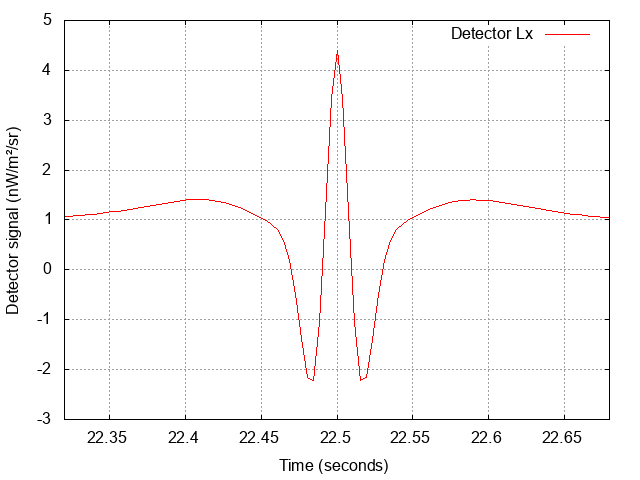
\includegraphics[width=0.48\textwidth,trim=8mm 0 0mm 0mm]{plots/tod000_stroke.png}
	\end{tabular}
	\caption{Noiseless simulated PIXIE time-ordered data for the Lx
	detector on various time scales. \emph{Top left}: A whole great-circle
	scan of the sky, starting at ecliptic coordinates $l=0\degree$,
	$b=0\degree$ and scanning in longitude. The two peaks are crossings
	of the galactic plane. \emph{Top right}: Zoom on the first 10 minutes.
	We see that the signal is modulated on 3 time-scales: The sky signal
	changes on minute time-scales due to the scan; the polarization is
	modulated on 15 second time-scales due to PIXIE's spin; and the
	signal is modulated on second time-scales by the mirror stroke.
	\emph{Bottom left}: Zoom on a single pixie spin. The slowly
	changing baseline is the DC signal, which PIXIE will not attempt
	to measure due to its suceptibility to 1/f noise. \emph{Bottom
	right}: Zoom on a single mirror half-stroke, centered on
	$\Delta t=0$. This is effectively a plot of the electric field's
	autocorrelation function at this position.}
\end{figure}

\begin{figure}
	\centering
	\hspace*{-15mm}\begin{tabular}{rm{56mm}m{54.4mm}m{56mm}}
		& \hspace{32mm}T & \hspace{32mm}Q & \hspace{32mm}U \\
		Input &
		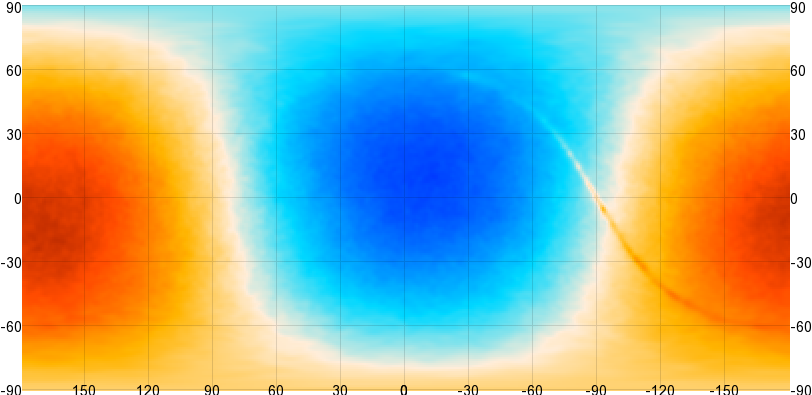
\includegraphics[height=28mm,clip,trim=0 8mm 7.5mm 0]{plots/sim_freqmap_58GHz_0_0.png} &
		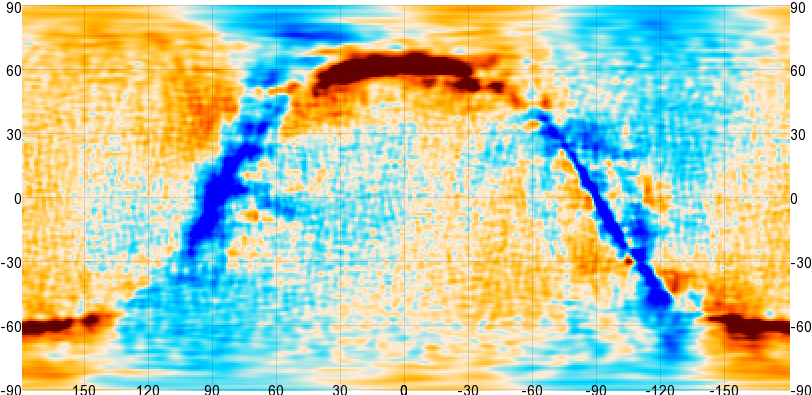
\includegraphics[height=28mm,clip,trim=7.5mm 8mm 7.5mm 0]{plots/sim_freqmap_58GHz_0_1.png} &
		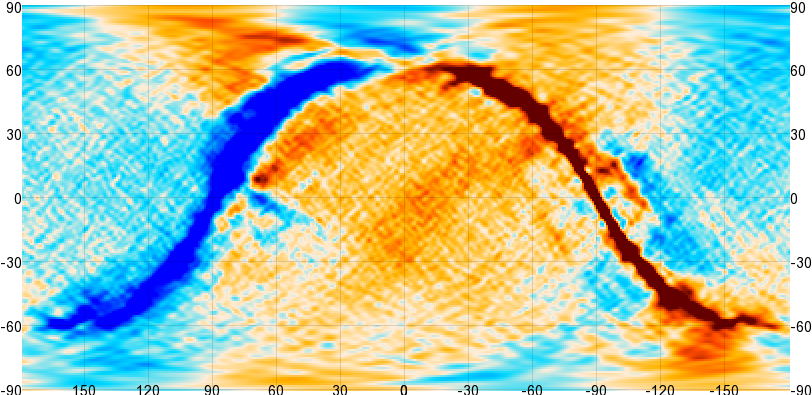
\includegraphics[height=28mm,clip,trim=7.5mm 8mm 0 0]{plots/sim_freqmap_58GHz_0_2.png} \\
		Error &
		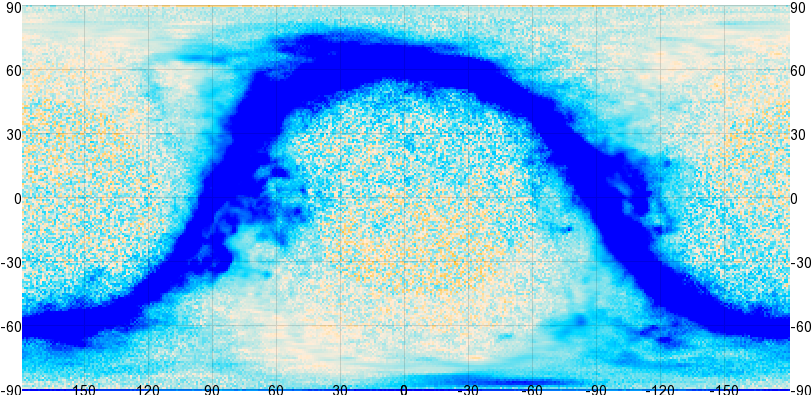
\includegraphics[height=29.7mm,clip,trim=0 0 7.5mm 0]{plots/map11_sub9_diff_58GHz_scaled_0.png} &
		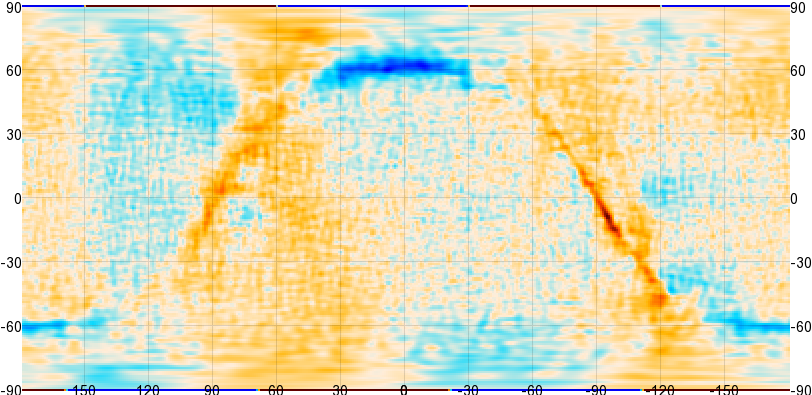
\includegraphics[height=29.7mm,clip,trim=7.5mm 0 7.5mm 0]{plots/map11_sub9_diff_58GHz_scaled_1.png} &
		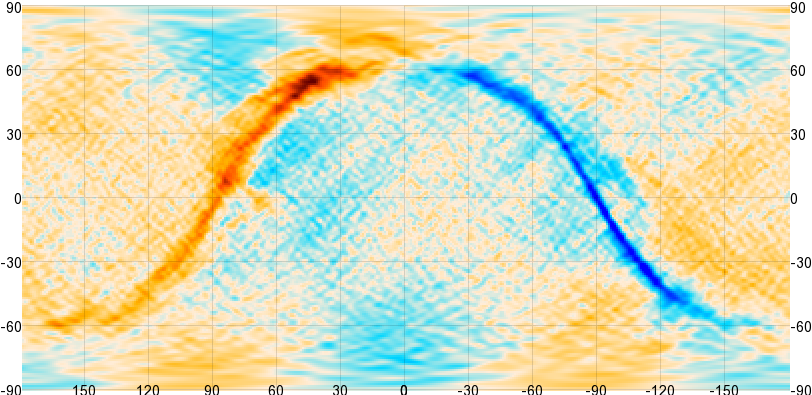
\includegraphics[height=29.7mm,clip,trim=7.5mm 0 0 0]{plots/map11_sub9_diff_58GHz_scaled_2.png}
	\end{tabular}
	\caption{Simulator/mapmaker spatial bias test.
		\emph{Top row}: The beam-smoothed simulated input map at 58 GHz.
			The color range is $\pm 400$ kJy/sr for T and $\pm 200$ Jy/sr for P.
		\emph{Bottom row}: Difference between the mapmaking output maps and
			input maps at the same frequency for a noise-less simulation.
			The color range is $\pm 1.7$ Jy/sr for T and $\pm 2.5$ mJy/sr for P.
			These represent the bias of the simulator-mapmaker combination.}
\end{figure}

\begin{figure}
	\centering
	\hspace*{-13mm}\begin{tabular}{m{59mm}m{59mm}m{59mm}}
		\hspace{30mm}Input & \hspace{20mm}Interpolations & \hspace{30mm}Residual \\
		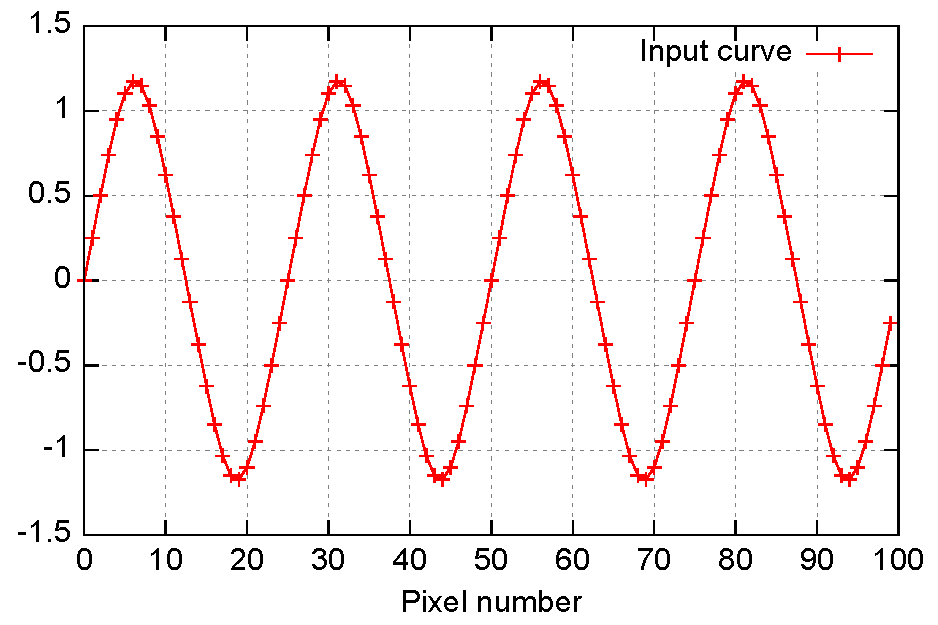
\includegraphics[height=43mm,clip,trim=0 0 0 0]{plots/subpixel_model_input.pdf} &
		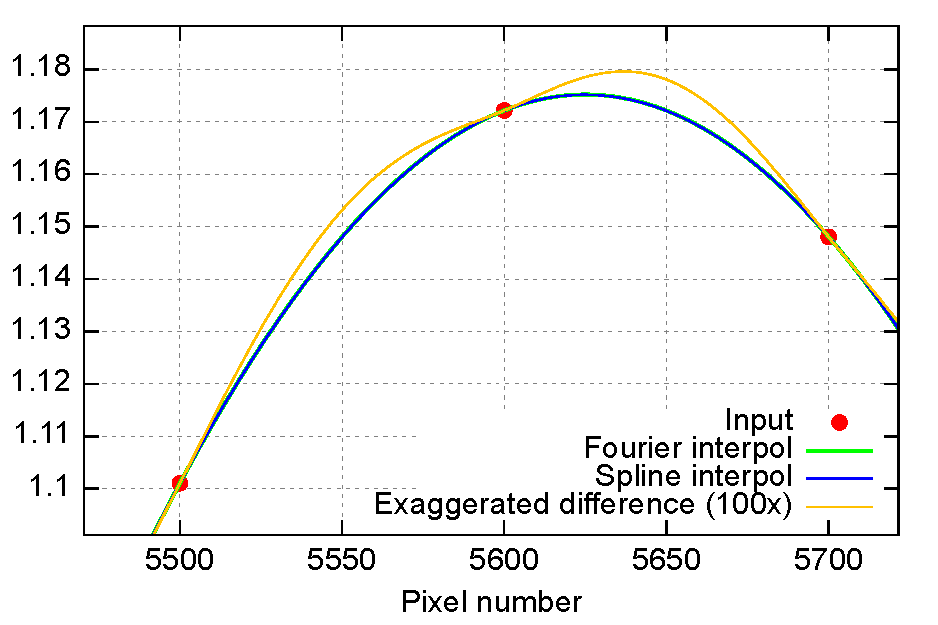
\includegraphics[height=43mm,clip,trim=0 0 0 0]{plots/subpixel_model_interpol.pdf} &
		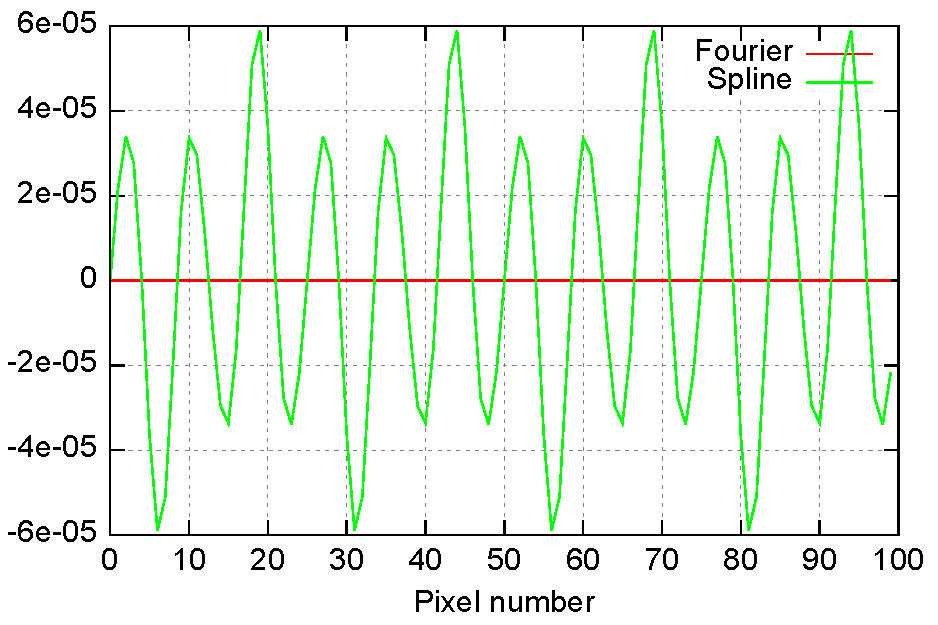
\includegraphics[height=43mm,clip,trim=0 0 0 0]{plots/subpixel_model_residual.pdf}
	\end{tabular}
	\caption{1-dimensional toy example of subpixel mismatch bias.
	\emph{Left}: The input data set, which is a densely sampled sine wave with
	25 points per wavelength. \emph{Middle}: Two models for the sub-pixel behavior
	of the data set (fourier and spline interpolation) disagree slightly.
	\emph{Right}: The residual after shifting the dataset right by half a sample
	(i.e. half-way between the red points in the middle panel) using fourier
	(red) and spline (green) interpolation, and then back again using fourier interpolation
	in both cases. When the forwards and backwards methods match, the result is biased.}
\end{figure}

\begin{figure}
	\centering
	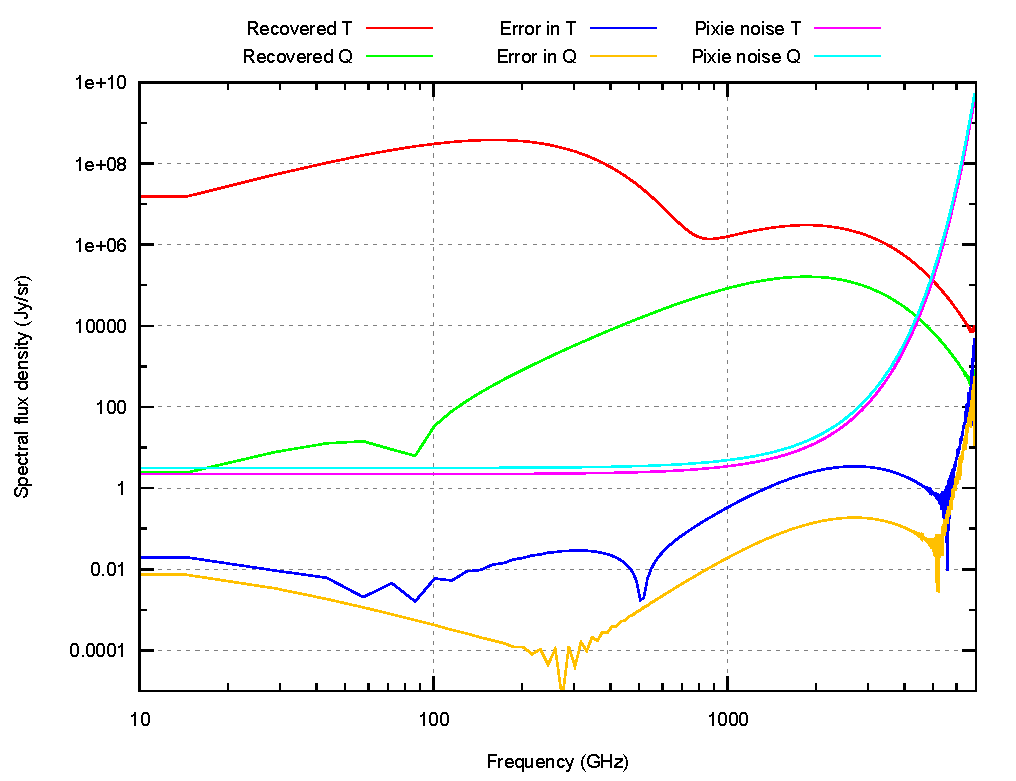
\includegraphics[width=0.8\textwidth]{plots/spec_error_abs_v4_log_log_sub9.pdf}
	\caption{Simulator/mapmaker spectral bias test. Recovered T and Q spectra and
	their errors for a noiseless simulation
	with 9 Gaussian quadrature subsamples per sample, compared to the pixie
	noise level. This is all for a single pixel at $l=0\degree$,$b=0\degree$.
	The U spectrum is similar to the Q one, but was left out to avoid clutter.
	The bias is $\sim 100$ times lower than the noise for $\nu<500$~GHz and
	$\sim 5$ times lower than the noise at the worst point at 2 THz. At 200
	Hz the bias is $\sim 10^{-10}$ of the signal in T and $\sim 10^{-6}$
	of the signal in P.}
\end{figure}

\begin{figure}
	\centering
	\hspace*{-2mm}\begin{tabular}{cc}
		T & Q \\
		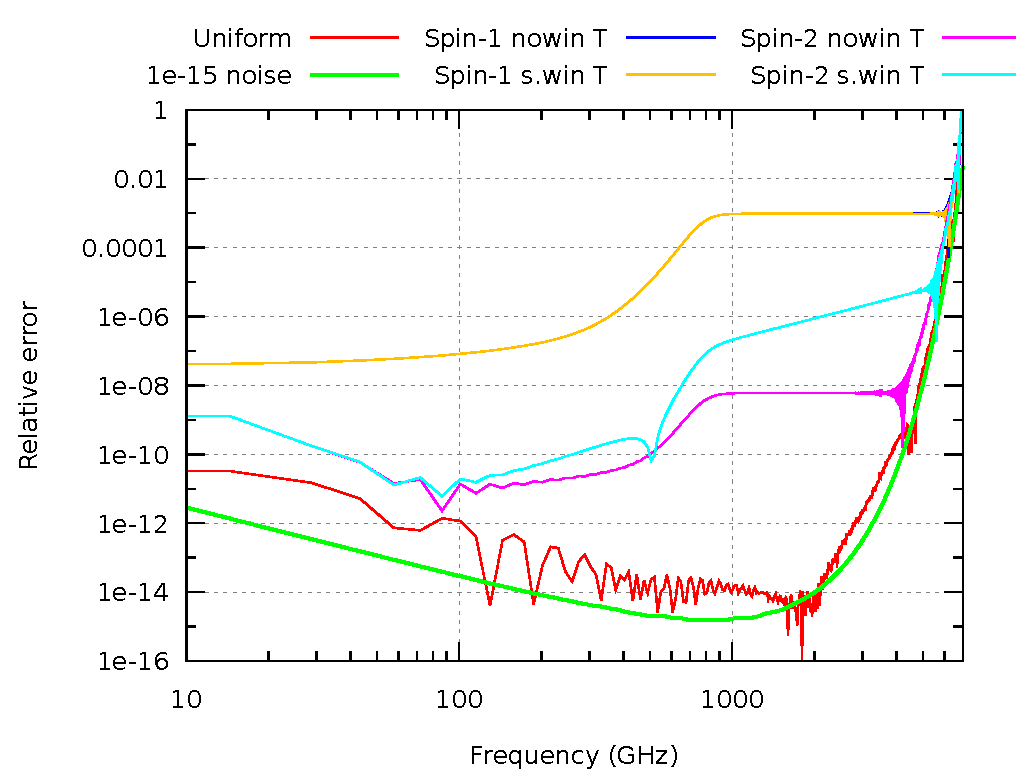
\includegraphics[height=70mm,clip,trim=0 0 0 0]{plots/spec_error_rel_v4_log_log_spin_win_T.pdf} &
		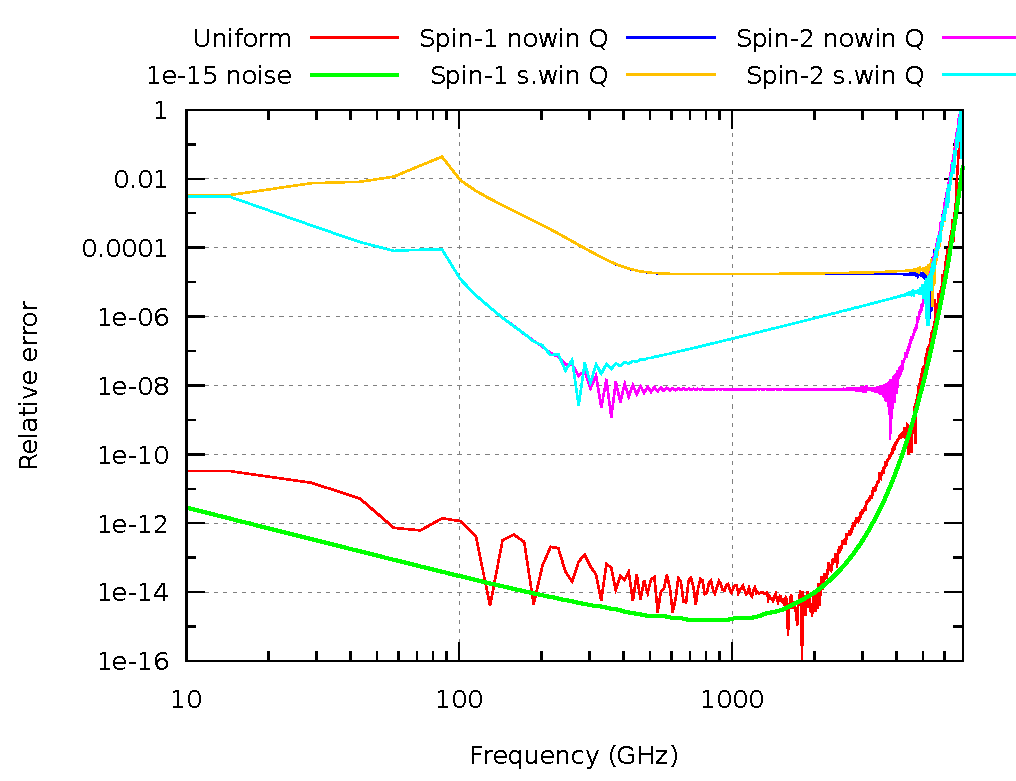
\includegraphics[height=70mm,clip,trim=30mm 0 0 0]{plots/spec_error_rel_v4_log_log_spin_win_Q.pdf}
	\end{tabular}
	\caption{The effect of sample window and fourier shift distance on the
	mapmaking bias. Both of these are examples of subpixel bias. The sample
	window error comes from the mismatch between the gaussian quadrature that is
	used to integrate the sample window and the fourier-space deconvolution that
	is used to remove it. It rises with frequency and is a $\sim 10^{-7}$ error
	at 1 THz. The fourier shift error comes from the mismatch between the
	high-res bicubic subpixel behavior of the sky in the simulator and the
	bandlimited fourier model used in the mapmaker. It has a surprisingly large
	dependence on the interpolation distance. Spin-1 fourier shifting has
	twice the interpolation distance of Spin-2 fourier shifting, but $10^3-10^4$
	times are large a bias. The red curve shows the error for a
	monopole-only sky when using no sample window, demonstrating
	that aside from subpixel biases the accuracy is close to double
	precision float error.}
\end{figure}

\end{document}
